\begin{centering} 
  \huge Development of TRatioPlot in ROOT \\ 
  \large \textbf{Paul Gessinger} \\ 
  \large CERN Summer Student project \\ 
\end{centering} 
\vspace{1.0cm}
\normalsize

\section{Status of ratio and similar plots in ROOT}

\noindent The ROOT data analysis and visualization framework is a software package which
is widely used in physics, especially in high energy physics. As the software became more
and more sophisticated, numerous improvements were made, and regularly, simplifications
for were achieved. 

Examples for this are the spectrum fitter and the stack facility.
A common visualization which has so far been lacking a direct implementation is the
ratio plot, as well as a few similar types of plots. The common element is a splitting
of the area into to sub areas, one of which contains the inputs, typically histograms,
whereas the other one displays the result of a calculation, as for example the result 
of a division of one histogram by the other.

While it was perfectly possible to create a plot like this in ROOT before, achieving 
a good looking result could be tedious, which led to a large number of people writing
automation on top of ROOT itself, that would take care of the process for them. The scope
and goal of my summer student project at CERN was to implement a class in ROOT itself,
that can take care of the most common types of calculations, and produces high quality
visuals. A key factor in the design was to ensure interactive usability of the class,
making it possible to explore calculation results more easily.

\begin{wrapfigure}{r}{0.4\textwidth}
  \centering
  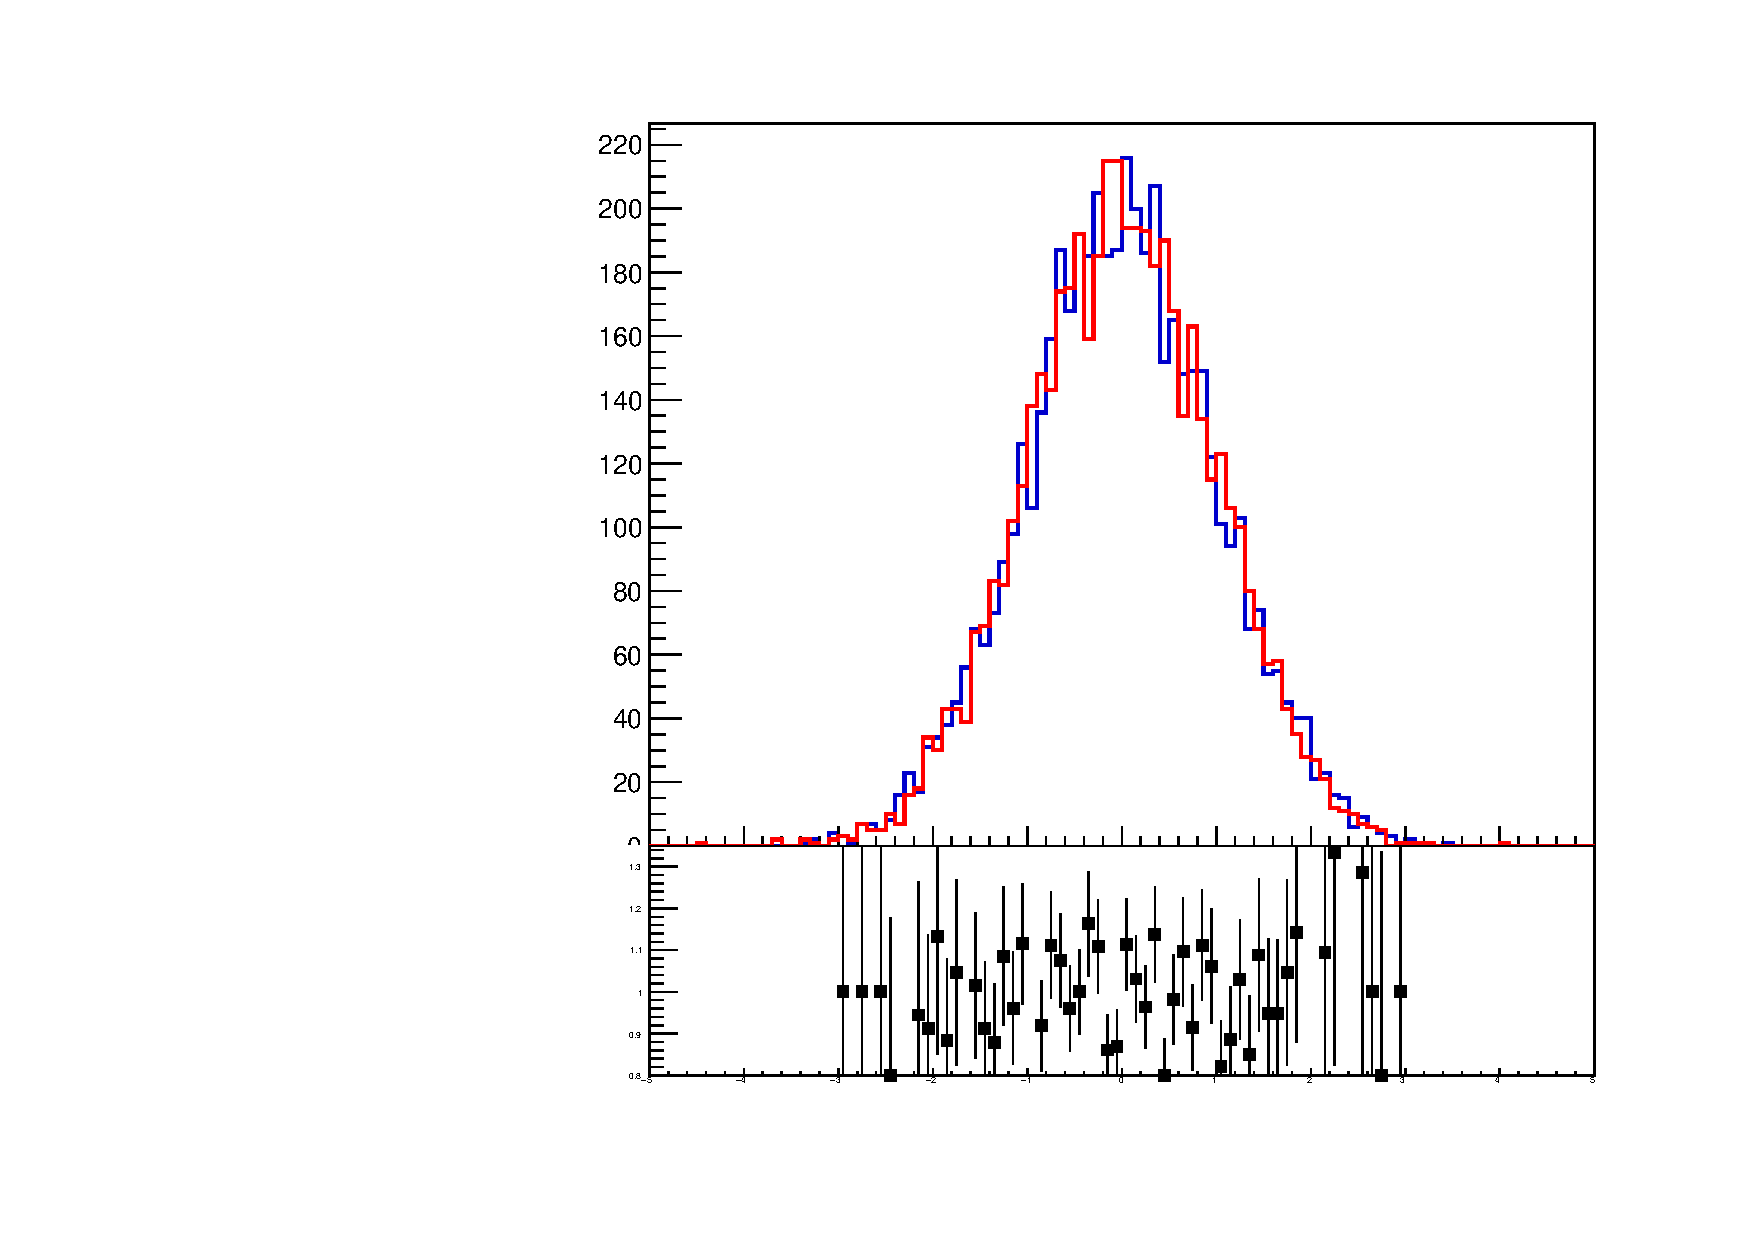
\includegraphics[width=1.0\linewidth]{assets/bad.pdf}
  \caption{Naive implementation of a ratio plot using two \texttt{TPad} objects.}
  \label{fig:bad}
\end{wrapfigure}

As can be seen \autoref{fig:bad}, directly using provided facilities in ROOT yields
unsactisfactory visual results. Axis labels are sized inconsistently, as the font sizes
are derived from the size of the pad within the parent. Showing axes titles would reveal
that here sizing is also inconsistent, as are the offsets from the axis itself. A major
problem for quality is the clipping of the 0 of the upper y axis. It results from the pads meeting,
and the lower pad cutting of the overflowing the lowest label of the upper y axis.

Not visible in the static image are the issues with interactivity this implementation has. When the user
views a ROOT plot, it is possible to manipulate the visuals using the mouse. For example 
the user can zoom in by clicking and dragging on one of the axes. It is also possible to switch
the display between a linear and a logarithmic scale. Clicking and dragging on the outer frame of the 
pads allows resizing the content frame. When performing any of these actions, the pads
react completely independently, meaning changes made to one of the pads is not reflected
on the other on. This can be problematic, specifically when attempting to use the zoom
feature to explore the content, since replicating the zoomed range precisely can prove a challenge.

\section{TRatioPlot}

The aforementioned shortcomings are attempted to be fixed by implementing a class called \texttt{TRatioPlot} and focussed on three main goals:

\begin{itemize}
  \item Produce high quality visuals with minimal setup
  \item Enable meaningful interactivity
  \item Implement most common calculations for these types of plots
\end{itemize}

\subsection{Output quality and size normalization}
Out of the box, when working with multiple pads, sizes are derived from the size of the pad. Therefore, if one
attempts to have consistent sizing, conversion factors have to be derived, or absolute sizing has to be utilized. While the latter is easily achievable, it also removes the useful benefits of having adaptable sizing. Say
you want to have a ratio type plot inside a positioned pad. In this case adaptable sizing will be useful to
produce readable output.

\begin{wrapfigure}{l}{0.4\textwidth}
  \centering
  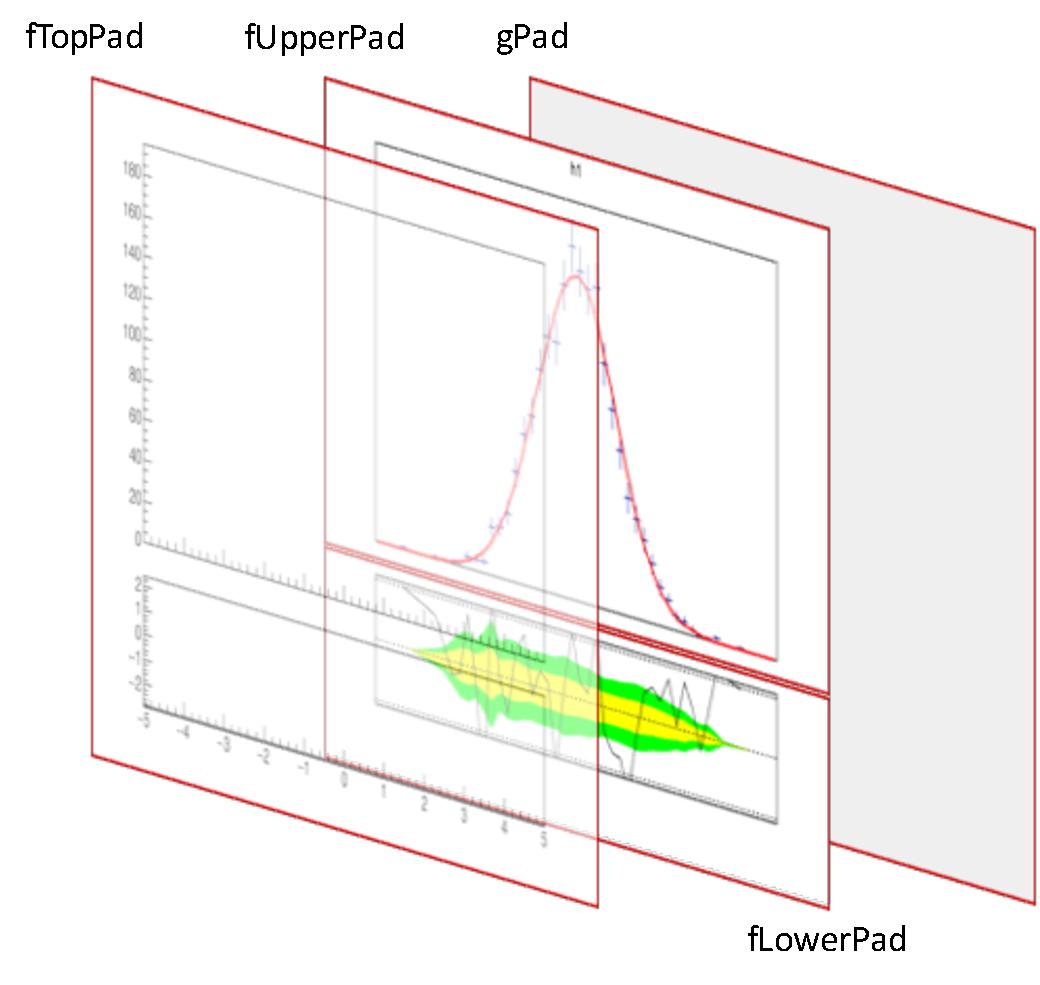
\includegraphics[width=1.0\linewidth]{assets/padstack.pdf}
  \caption{\texttt{TPad} structure of the new \texttt{TRatioPlot} class.}
  \label{fig:padstack}
\end{wrapfigure}

In order to preserve the sizing mechanism, the pad structure of the class was adjusted as can be seen
in \autoref{fig:padstack}. When creating
an instance of the class, it will create three \texttt{TPad} objects inside the currently active pad.
Two pads receive the input histograms and the output graphs respectively. Drawing of axes is disabled
when drawing objects in these pads. The draw option "A" of \texttt{TH1} prevents visible axes, while
retaining the ability to interact with them. The draw option "I" achieves the same when drawing
\texttt{TGraph}. The pad marked by \emph{fTopPad} receives all the visual axes. Since all of them are drawn
in one pad spanning the full dimensions of the containing pad, label and title sizes and offsets are consisten
between them. Properties for the visual axes are first imported from the corresponding axes of the drawn
objects, and changed where necessary. For example, the class always hides the axes labels and title on the upper x axis. The margins of the pads are synchronized. Using setters on \texttt{TRatioPlot}, margins that
should be identical can be set at the same time. Another setter can be used to determine the separation
between the upper and the lower plot, while yet another one determines the point at which the two pads
meet. Draw options given to \texttt{TRatioPlot} can enable and disable visual features, they are listed
in \autoref{tab:drawopt}.

\begin{table}[hb]
  \centering
  \begin{tabular}{l|l}
    Draw option & Description \\
    \hline
    grid / nogrid & enable (default) or disable drawing of dashed lines on lower plot \\
    hideup & hides the first label of the upper axis if there is not enough space \\
    fhideup & always hides the first label of the upper axis \\
    hidelow (default) & hides the last label of the lower axis if there is not enough space \\
    fhidelow & always hides the last label of the lower axis \\
    nohide & does not hide a label if there is not enough space \\
    noconfint & does not draw the confidence interval bands in the fit residual case \\
    confint & draws the confidence interval bands in the fit residual case (default) \\
  \end{tabular}  
  \caption{Draw options for \texttt{TRatioPlot}.}
  \label{tab:drawopt}
\end{table}

\noindent
The class will hide y axis labels once the pads are closer than a certain threshold, to prevent clipping
and also overlapping of axis labels. The lower plot contains dashed lines, promoting points of interest,
such as the value 1 in a ratio. This behaviour can be turned off via a draw options, however it is 
also possible to set the y positions of an arbitrary number of dashed lines manually using the
\texttt{TRatioPlot::SetGridlines()} method, by passing an array of y values.

\subsection{Interactive manipulation}

In order to support the functionality of ROOT to view and manipulate most structures interactively,
care has to be taken. Without the use of \texttt{TRatioPlot}, modifying one of the pads used for
display will not trigger a corresponding change in the other one. This is undesirably for obvious reasons.
\texttt{TRatioPlot} aims to fix this problems. Using the the Signal/Slot mechanism, it is possible 
to react to changes, that are triggered and processed elsewhere. The class connects to three signals
from the contained pads, \emph{RangeAxisChanged}, \emph{Resized} and \emph{UnZoomed}, only the first
of which used to exist. It was called whenever the actual range of the axis changed, as the name
indicates. \texttt{TPad} was modified to also emit this signal when on of the axes is switched
between linear and logarithmic mode. The second signal is emitted after the pad has responded to 
interactive resizing by clicking and dragging, which means that it already contains the updated
coordinates. The last signal was added and is emitted when selecting the unzoom entry in the context
menu of an axis. 

Using slots for these signals, \texttt{TRatioPlot} can react to changes made by the user. The class
determines which element has changed, by comparing values to reference values stored inside the 
class after a previous change, or by determining the sender of the signal. It then updates internal
references accordingly, and sets the corresponding properties on the relevant other objects. For instance,
zooming updates the unchanged pad's axis to the one that was modified by clicking and dragging. A subsequent
paint picks up these changes, and renders the updated histograms and graphs, while also updating the
graphical axes that the class manages itself. Aside from axis ranges, this method is applied to changing
pad margins, logarithmic or linear axis setting for the x axis, as well as the point where the pads meet.

\subsection{Calculation modes}
A large number of calculations can be performed, that lend itself to visualization in the manner that
this class tries to provide. Effectively, any calculation whose output shares the x axis with this
inputs benefits from display in this way. While implementing all calculations in such a class would
be out of scope for a rather generic solution, it is still useful to have prebuild facilities for 
a few of the most used calculation modes. 

\textbf{Ratio of two histograms}\\
The simplest case is the division of one histogram by another one. This can be performed in multiple
ways using \texttt{TRatioPlot}. The default, when instantiating the class simply with two histograms,
is to delegate the calculation to \texttt{TGraphAsymmErrors::Divide}, while passing it the option
\emph{pois}, which makes use of the poisson error for each of the bins, and yields asymmetric errors on
the output. Another option is using the method \texttt{TH1::Divide}, which yields symmetric errors
and can be invoked using the option \emph{divsym} in the constructor.

\textbf{Difference of two histogram}\\
The second use case is two calculate the absolute difference between the two passed histograms.
This can be achieved by giving the option \emph{diff} when instantiating. Another possibility is 
to calculate the difference between the histograms, and then divide by the statistical uncertainty of
the first histogram. This mode can be invoked by using the option \emph{diffsig}. Two possibilities
exist for the source of the uncertainty, which can be selected using an additional option. The default is
to use the method \texttt{TH1::GetBinError}, which always yields symmetric uncertainties. By passing
the option \emph{errasym} one can have the calculation use the computed errors obtained through
\texttt{TH1:GetBinErrorUp} and \texttt{TH1::GetBinErrorLow}, which can yield asymmetric errors. Depending
on whether the first histogram's bin content is above the second histogram one's, the up or low
error is used. To ensure correct calculation, \texttt{TH1::SetBinErrrorOption} must be called on the
input histogram.

\textbf{Fit residual}\\
When fitting, it is often interesting to have a graphical representation of the quality and goodness
of a fit. To provide this, \texttt{TRatioPlot} can calculate the fit residual, which is the difference
between the actual bin content, and the corresponding fitted function value at the center of the bin, divided
by the uncertainty. Different uncertainties can be used, firstly, both options described in the previous
section are available, while a third option, \emph{errfunc}, enables the use of the square root of the
function value as the uncertainty. The fit residual calculation can be invoked by using the constructor
of the class which only accepts a single histogram. It is expected that the given histogram contains
one element in it's list of fitted functions. In addition to the fit residual itself, the class 
will also present the $1\sigma$ and $2\sigma$ confidence intervals. Drawing of these bands can be 
configured by using the draw options found in \autoref{tab:drawopt}.


\section{Example output}
This section shows three example outputs, that can be achieved using \texttt{TRatioPlot}. The corresponding
code can be found in the appendix in an abbreviated form.

\begin{figure}
  \begin{subfigure}{0.5\linewidth}
    \centering
    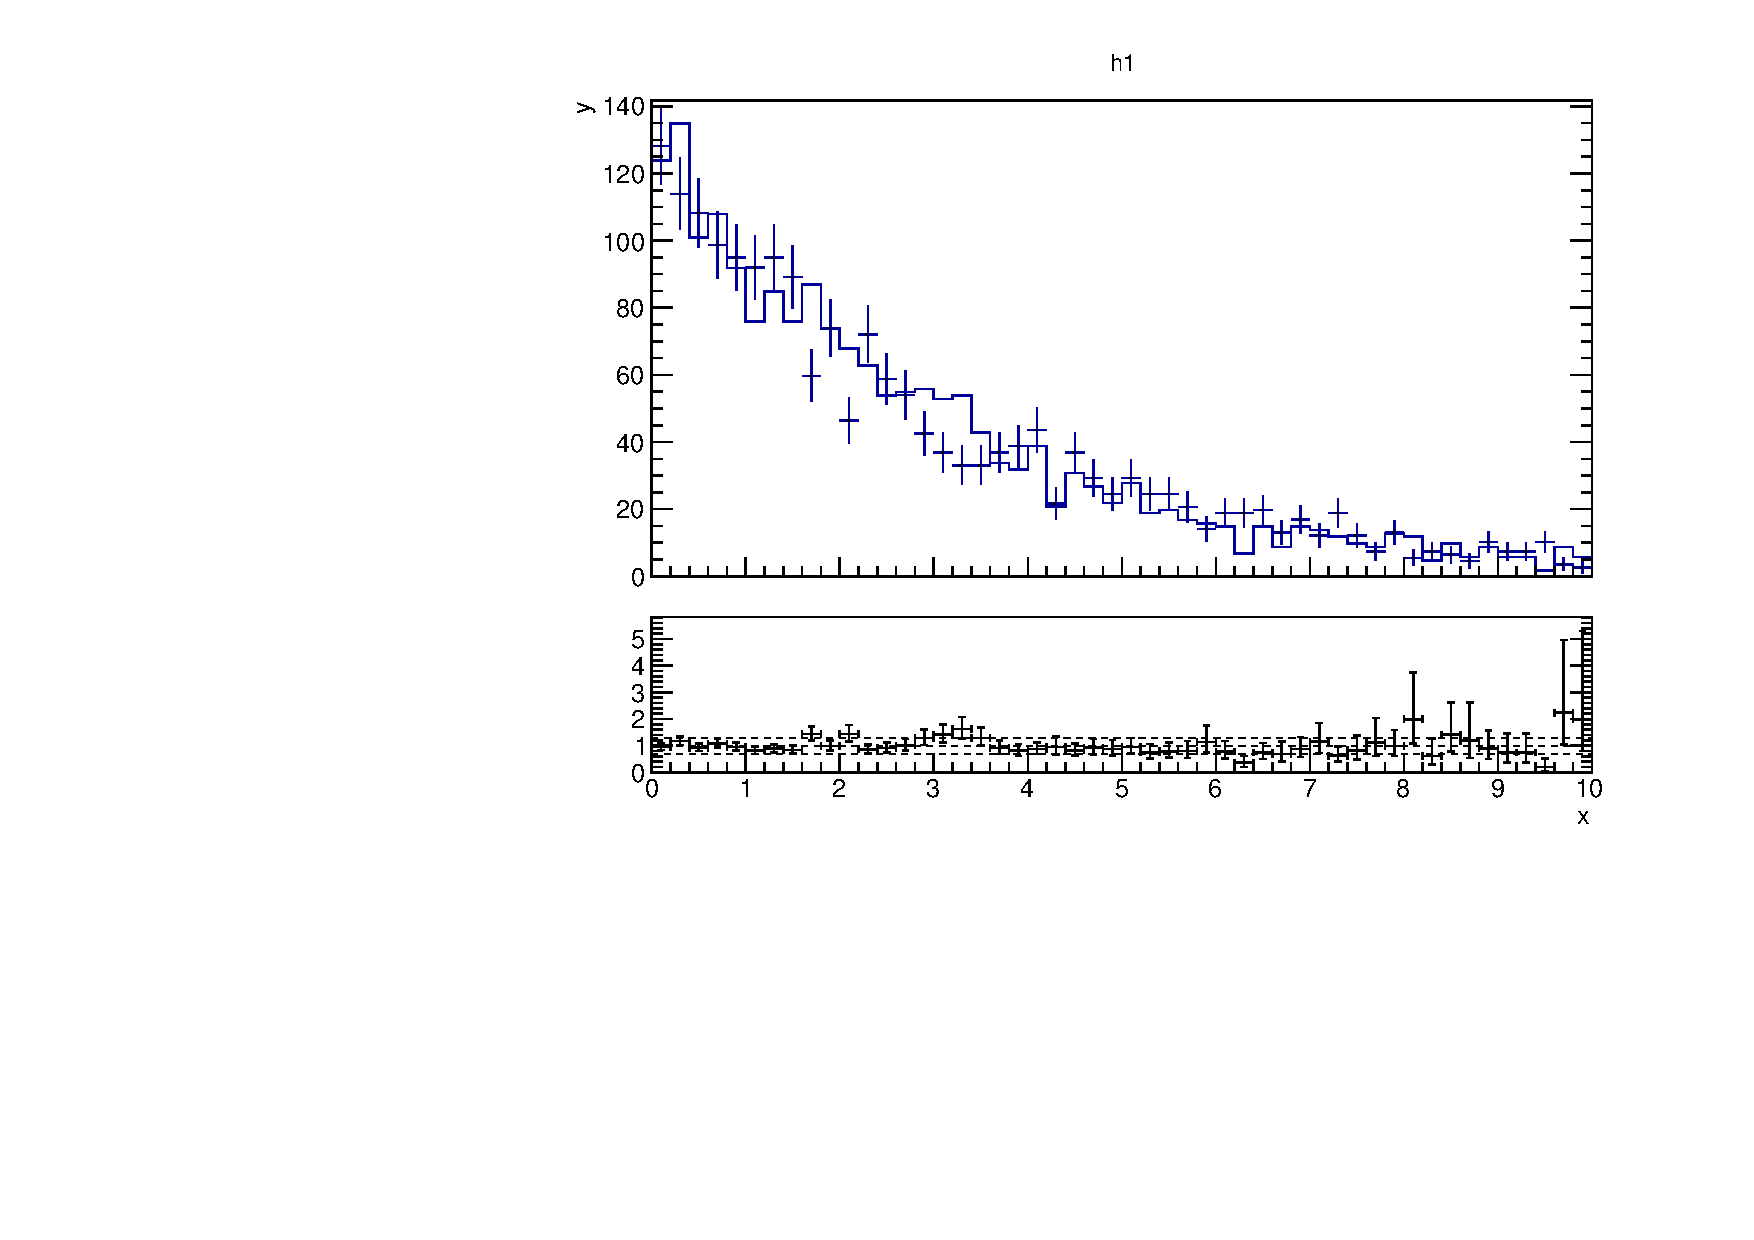
\includegraphics[width=1.0\linewidth]{assets/tut1.pdf}   
    \caption{Ratio of two histograms. (see \autoref{lst:ratio} for code)}
    \label{fig:ratio}
  \end{subfigure}
  \begin{subfigure}{0.5\linewidth}
    \centering
    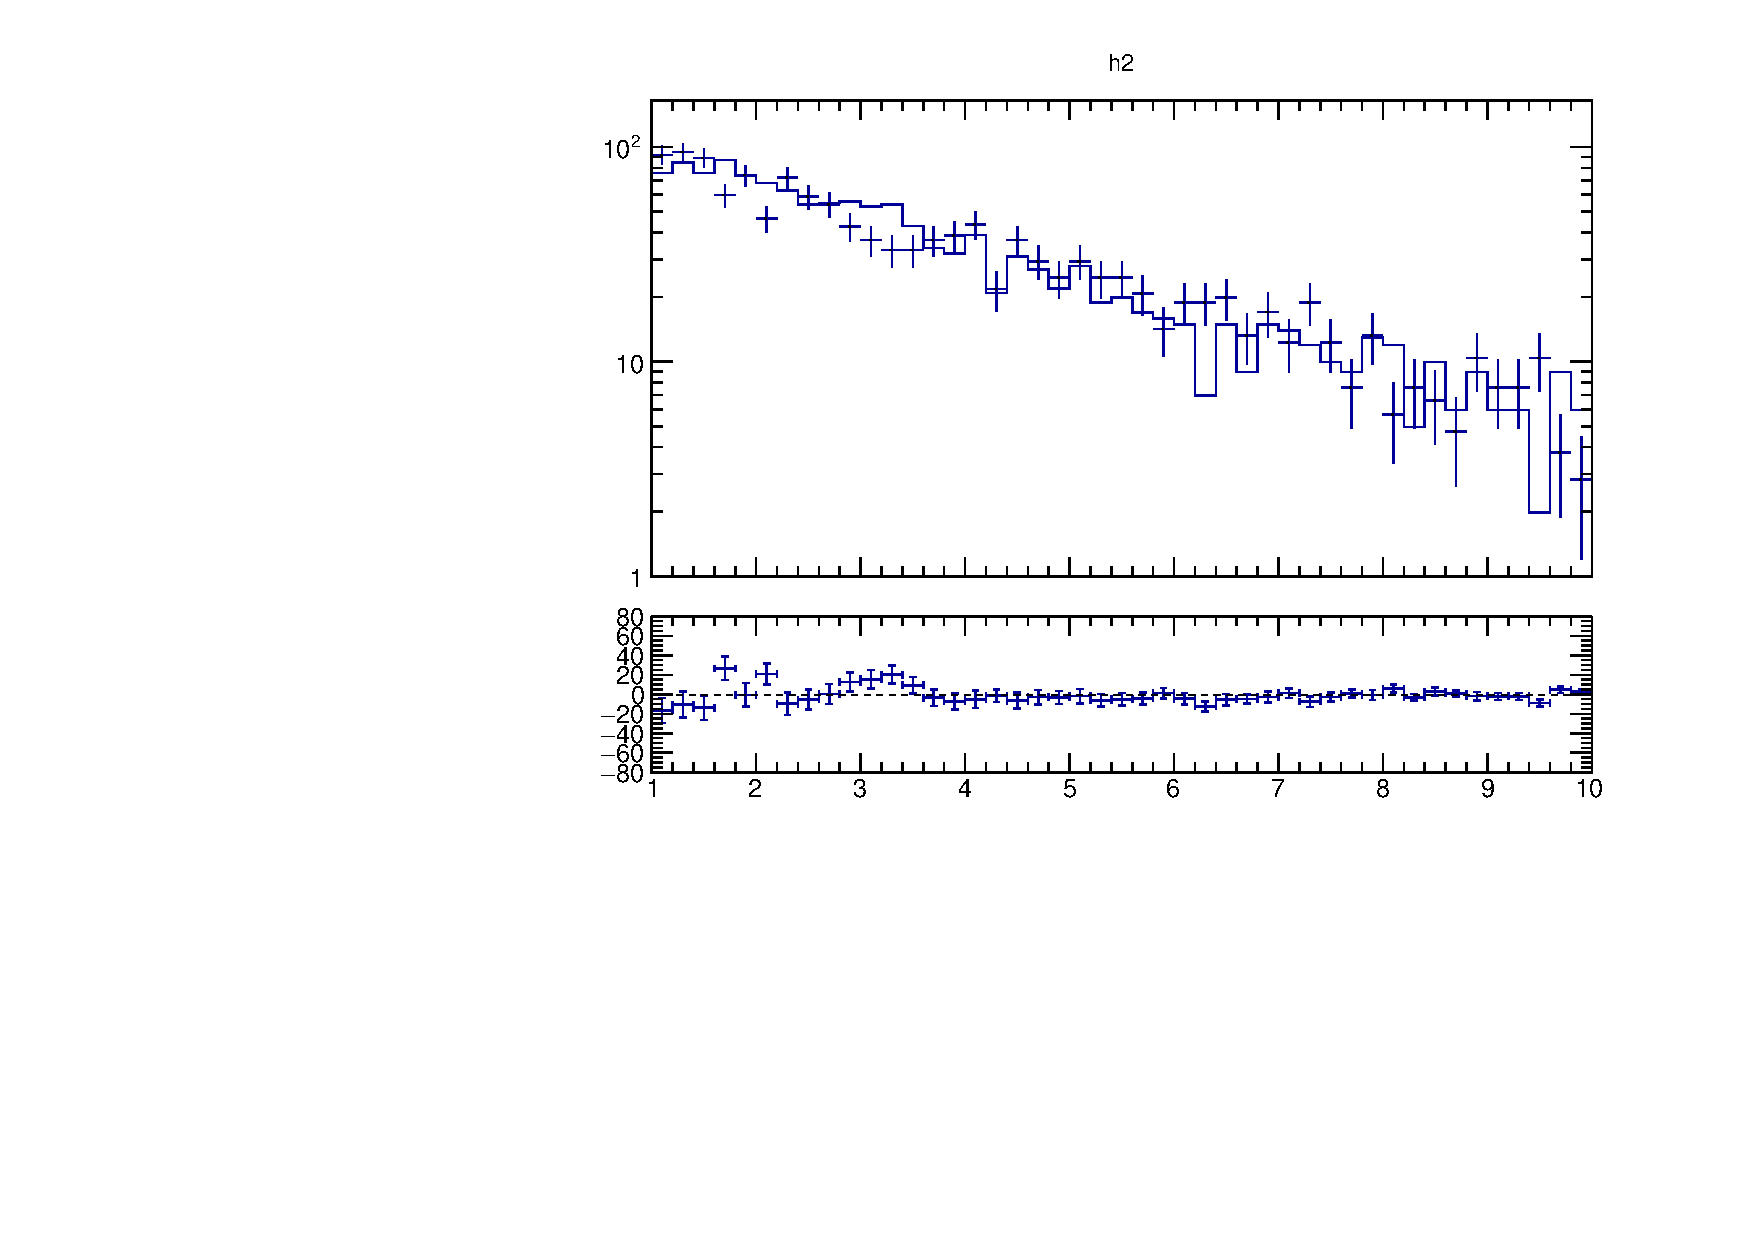
\includegraphics[width=1.0\linewidth]{assets/diff.pdf}  
    \caption{Difference between two histograms. (see \autoref{lst:diff} for code)}
    \label{fig:diff}
  \end{subfigure}
  \begin{subfigure}{0.5\linewidth}
    \centering
    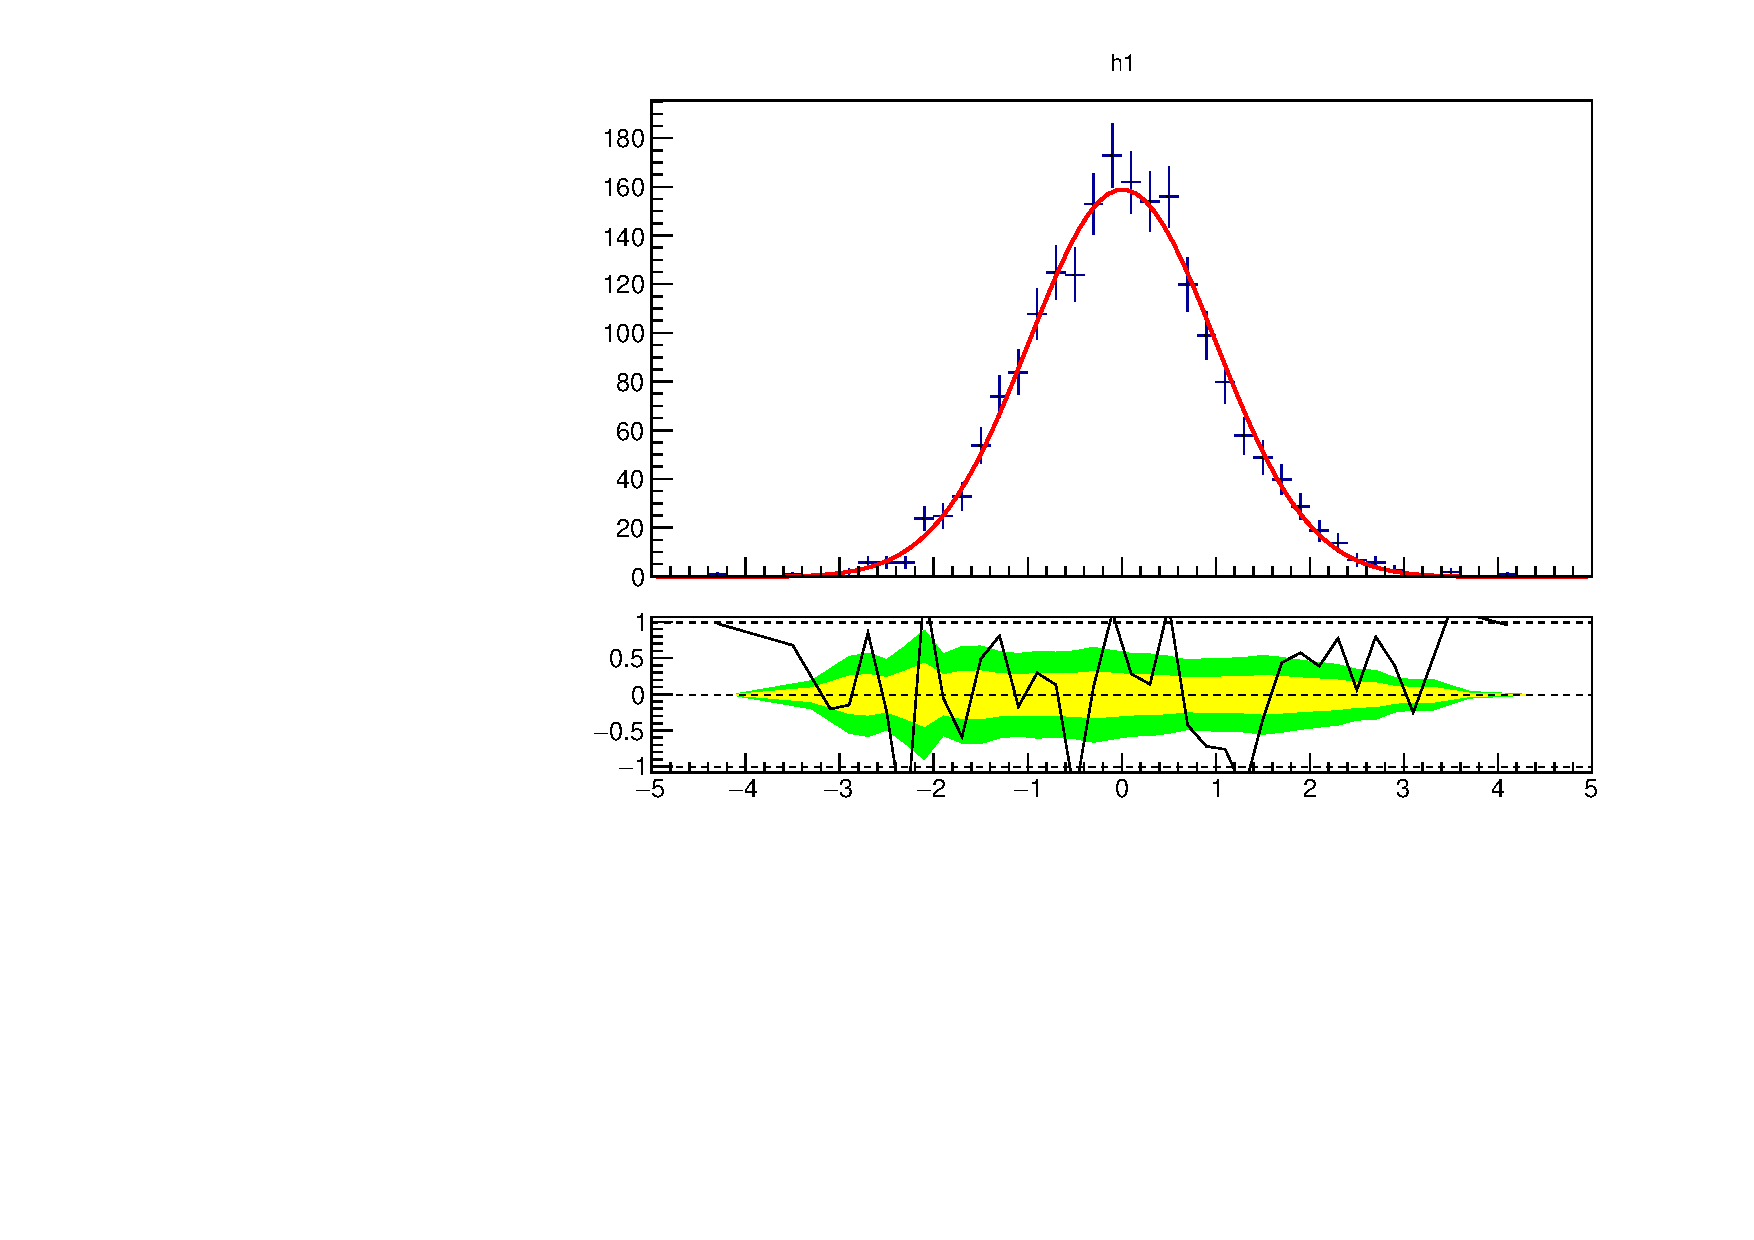
\includegraphics[width=1.0\linewidth]{assets/single.pdf} 
    \caption{Residual of a fit to a histogram. (see \autoref{lst:fitres} for code)}
    \label{fig:fitres}
  \end{subfigure}
\end{figure}

\autoref{fig:ratio} shows a simple ratio of two histograms, \autoref{fig:diff} shows the difference
between two histograms and \autoref{fig:fitres} shows the case of a fit residual to a histogram.

\section{Summary}
During the CERN Summer Student project, a class called \texttt{TRatioPlot} was integrated into
the ROOT framework, than can greatly simplify common plotting tasks, and potentially save a lot
of time spend by a lot of people on reimplementing the same functionality. The class can produce
high quality visualization of ratio and similar plots. It also enables interactivity for these
kinds of plots for the first time in ROOT. Additionally, the class implements a number of 
commonly performed calculations typically shown in the relevant manner. This means that producing
these plots will require less code in most cases. Customization of the output is also improved,
since the class provides new facilities to operate on coupled display pads at the same time.

\clearpage

\begin{appendix}
  \section{Appendix}
  \begin{figure}[h]
    \lstinputlisting{assets/ratioplot1.C}
    \caption{Simple example for a ratio.}
    \label{lst:ratio}
  \end{figure}
  
  \begin{figure}[h]
    \lstinputlisting{assets/diff_logxy.C}
    \caption{Simple example for a difference of two histograms.}
    \label{lst:diff}
  \end{figure}
  
  \begin{figure}[h]
    \lstinputlisting{assets/single.C}
    \caption{Simple example for a fit residual.}
    \label{lst:fitres}
  \end{figure}
  \printbibliography
\end{appendix}
